%!TEX root = ../template.tex
%%%%%%%%%%%%%%%%%%%%%%%%%%%%%%%%%%%%%%%%%%%%%%%%%%%%%%%%%%%%%%%%%%%%
%% chapter3.tex
%% NOVA thesis document file
%%
%% Chapter with a short latex tutorial and examples
%%%%%%%%%%%%%%%%%%%%%%%%%%%%%%%%%%%%%%%%%%%%%%%%%%%%%%%%%%%%%%%%%%%%

\typeout{NT FILE chapter3.tex}%

\chapter{Work Plan}
\label{cha:work_plan}

This thesis combines, among other topics, two important fields of study: radar technology and machine learning.

It is therefore structured into several tasks that are designed to meet its objective. This chapter outlines the strategy, timeline, and steps involved, which helps to organize the research activities, allocate resources and maintain focus on the goal of the project. An overview of that goal was defined in Section \ref{sec:goals}, and in the following sections several tasks and milestones are defined to be achieved during the course of the study.

\section{Task Description} % (fold)
\label{sec:task_description}
The work plan for this thesis includes the following tasks:

\begin{enumerate}     

\item \textbf{Overview of related work}

This task includes the study and comprehension of Frequency Modulation Continuous Wave active radio frequency sensing. In a further step, the task includes the identification of popular machine-learning techniques adopted in the literature to address the topic of human posture and motion classification, as well as the type of features involved in the classification process and the signal processing methods to compute them

\item \textbf{Real-time Data Visualization and Features}

This task involves the experimentation of different visualization tools capable of showing the dynamic behaviour of different features computed in real-time. The goal is to obtain a visual assessment of hypothetical features to adopt, how they change over time, and validate their adequacy for different types of motion.

\item \textbf{Identification and Characterization of Different features}

In this task, several datasets will be obtained to identify potential features that better represent the data’s information. The analysis might include an initial characterization of the data’s statistical properties and in a subsequent step, the identification and assessment of various types of features adopted in the classification process.

\item \textbf{Classification}

This task handles the development of classification methodologies to identify the sensed context with high accuracy and in a short period of time. The implementation of a demonstration prototype is a secondary goal, once the most appropriate classification methodology has been identified. 

\item \textbf{Performance Evaluation}

This task evaluates the performance of the solutions proposed in tasks T1 to T4. During T1 the evaluation of related works takes place. The identified features and classification methods explored in tasks T2 and T3 will be compared by assessing the performance of each combination in real-time operation.

\item \textbf{Thesis Writing}

This task includes the reporting activities in initial drafts to describe the proposed solutions and the performance results achieved in the first step. The documents will be updated over time to contain all the steps developed during the working period and, at the final stage, they include all the material required for each chapter of the MSc dissertation. This task can might also include the reporting of the achievements in a scientific paper.  

\end{enumerate}


\section{Schedule} % (fold)
\label{sec:schedule}
\begin{figure}[ht]
    \centerline{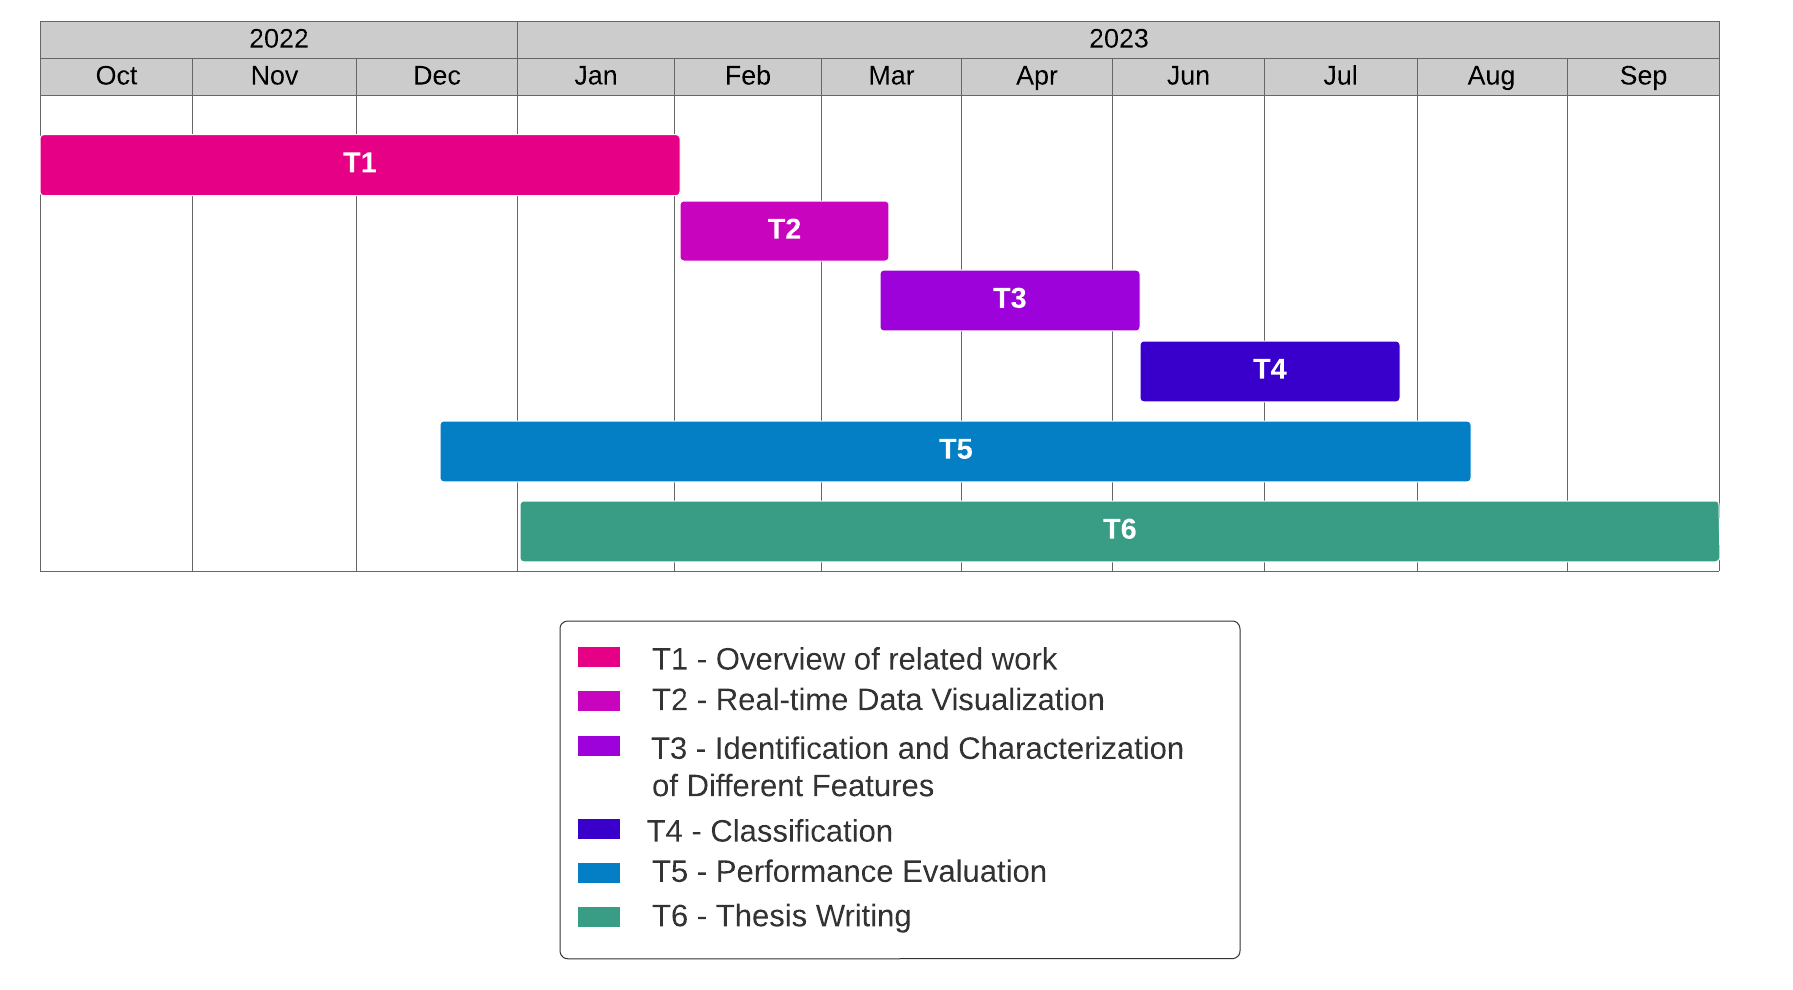
\includegraphics[scale = 0.25]{Chapters/Figures/GanttChart.png}}
    \caption{Gantt Chart for the timeframe of this thesis work plan.}
    \label{fig:schedule}
\end{figure}
A Gantt chart with the time schedule for this thesis is presented in figure \ref{fig:schedule}. It provides a visual representation of the thesis schedule that displays the start and finish dates predicted for the tasks. 


The practical work will begin in February with the second task. The graph also shows that thesis writing began in January and will continue until September, owing to the fact that this report already contains information for some chapters of the thesis. 
Although the writing task is indicated in the chart as concluding in September, it should be noted that it will continue until all issues related to the growth of this thesis have been described. Although September 2023 is the stated deadline, it would be preferable and expected for the task to be completed sooner.
Since it is possible to infer the performance of other studies dissected during T1 as well as the performance of the solution suggested in this thesis constructed over Tasks 2 and 3, the performance evaluation (T4) task runs concurrently with Tasks T1 to T3.

